\section{Sigmoidal functions}
\textbf{Definition 1.} A function $\sigma: \mathbb{R}\rightarrow [0,1]$ is called sigmoidal if

$$
\lim_{x\rightarrow -\infty}\sigma(x)=0, \qquad \lim_{x\rightarrow \infty}\sigma(x)=1.
$$

\textbf{Definition 2.} Let $n$ be a natural number. We say that an activation function $f:\mathbb{R} \rightarrow \mathbb{R}$ is $n$-discriminatory if the only signed Borel measure $\mu$ such that

$$
\int f(y\cdot x+\theta)d\mu(x)=0, \quad \forall y\in\mathbb{R}^n, \theta\in \mathbb{R},
$$

is the zero measure.

\textbf{Definition 3.} We say an activation function $f:\mathbb{R} \rightarrow \mathbb{R}$ is discriminatory if it is $n$-discriminatory for any $n$.

\textbf{Remark 1.} A discriminatory function $\sigma$ is volumetrically non-destructive when it acts on linear transformations of input.


\subsection*{Activation functions}
\textbf{Step function}

$$\sigma(t)=
\left\{
  \begin{array}{ll}
  1, & t\geq 0 \\
  0, & t<0
  \end{array}
\right.
$$

\textit{Cons}

\begin{itemize}
  \item It cannot provide multi-value outputs—for example, it cannot be used for multiclass
classification problems.
  \item The gradient of the step function is zero, which causes a hindrance in the
backpropagation process.
\end{itemize}

\textbf{Linear}

$$\sigma(t)=t$$

\textit{Cons}

\begin{itemize}
  \item It’s not possible to use backpropagation as the derivative of the function is a
constant and has no relation to the input x.
  \item All layers of the neural network will collapse into one if a linear activation
function is used. No matter the number of layers in the neural network, the last
layer will still be a linear function of the first layer. So, essentially, a linear
activation function turns the neural network into just one layer.
\end{itemize}

\textbf{Sigmoid}

$$\sigma(t)=\displaystyle\frac{1}{1+\exp(-t)}$$

\textit{Pros}

\begin{itemize}
  \item It is commonly used for models where we have to predict the probability as an
output. Since probability of anything exists only between the range of 0 and 1,
sigmoid is the right choice because of its range.
  \item The function is differentiable and provides a smooth gradient, i.e., preventing
jumps in output values. This is represented by an S-shape of the sigmoid activation function.
\end{itemize}

\textit{Cons}

\begin{itemize}
  \item As we can see from the Figure, the gradient values are only significant for
range -4 to 4, and the graph gets much flatter in other regions.
It implies that for values greater than 4 or less than -4, the function will have very
small gradients. As the gradient value approaches zero, the network ceases to learn
and suffers from the \textit{Vanishing gradient problem}.
  \item The output of the logistic function is not symmetric around zero. This makes the training of the
neural network more difficult and unstable.
\end{itemize}

\textbf{Tanh}

$$\sigma(t)=\displaystyle\frac{\exp(t)-\exp(-t)}{\exp(t)+\exp(-t)}$$

\textit{Pros}

\begin{itemize}
  \item The output of the tanh activation function is Zero centered; hence we can
easily map the output values as strongly negative, neutral, or strongly positive.
  \item Usually used in hidden layers of a neural network as its values lie between -1 and 1; therefore, the mean for the hidden layer comes out to be 0 or very close to
it. It helps in centering the data and makes learning for the next layer much
easier.
\end{itemize}

\textit{Cons}

\begin{itemize}
  \item Also tanh faces the problem of \textit{vanishing gradients} similar to the
sigmoid activation function. Plus the gradient of the tanh function is much steeper as
compared to the sigmoid function.
Although both sigmoid and tanh face vanishing gradient issue, tanh is
zero centered.
Therefore, in practice, tanh nonlinearity is always preferred to sigmoid
nonlinearity.
\end{itemize}

\textbf{ReLU}

$$\sigma(t)=\max(0,t)$$

\textit{Pros}

\begin{itemize}
  \item Since only a certain number of neurons are activated, the ReLU function is far
more computationally efficient when compared to the sigmoid and tanh
functions.
  \item ReLU accelerates the convergence of gradient descent towards the global
minimum of the loss function due to its linear, non-saturating property.
\end{itemize}

\textit{Cons}

\begin{itemize}
  \item The negative side of the graph makes the gradient value zero. Due to this reason,
during the backpropagation process, the weights and biases for some neurons are
not updated. This can create dead neurons which never get activated.
All the negative input values become zero immediately, which decreases the
model’s ability to fit or train from the data properly.
\end{itemize}

\textbf{Parametric ReLU}

$$\sigma(t)=\max(at,t), \quad a>0$$

Parametric ReLU (PReLU) is an extension of Leaky ReLU (LReLU). While both introduce a slope for negative values to keep the gradient alive, the key difference is that PReLU has a learnable parameter \(a\) for the slope, whereas LReLU uses a fixed small value for \(a\). \\  This learnable parameter in PReLU allows the activation function to adapt to the data during training, providing more flexibility compared to LReLU.

\textit{Pros}

\begin{itemize}
\item Like ReLU, Parametric ReLU (PReLU) allows for efficient computation and mitigates the vanishing gradient problem for positive values. Additionally, it enables backpropagation for negative input values by maintaining a non-zero gradient, preventing dead neurons.
\item The parameter \(a\) is learnable, allowing the activation function to adapt to the data during training, potentially improving model performance.
\end{itemize}

\textit{Cons}

\begin{itemize}
\item Predictions for negative input values may be less consistent due to the learnable nature of the parameter \(a\).
\item If the learned parameter \(a\) is small, the gradient for negative values might be small, potentially making the learning process slower for those parameters.
\end{itemize}
\textbf{ELU (Exponential Linear Unit)}

$$
\sigma(t)=
\left\{
  \begin{array}{ll}
  t, & t\geq 0 \\
  \alpha(\exp(t)-1), & t<0
  \end{array}
\right.  
$$

\textit{Pros}

\begin{itemize}
  \item ELU becomes smooth slowly until its output equal to $a$ whereas RELU sharply smoothes.
  \item Avoids dead ReLU problem by introducing log curve for negative values of
input. It helps the network nudge weights and biases in the right direction.
\end{itemize}

\textit{Cons}

\begin{itemize}
  \item It increases the computational time because of the exponential operation
included
  \item No learning of the $a$ value takes place
  \item Exploding gradient problem
\end{itemize}

\textbf{Swish}

$$\sigma(t)=\displaystyle \frac{t}{1+\exp(-\beta t)}, \quad \beta \geq 0$$

\textit{Pros}

\begin{itemize}
  \item Swish is a smooth function that means that it does not abruptly change
direction like ReLU does near x = 0. Rather, it smoothly bends from 0 towards
values $< 0$ and then upwards again.
  \item Small negative values were zeroed out in ReLU activation function. However,
those negative values may still be relevant for capturing patterns underlying
the data. Large negative values are zeroed out for reasons of sparsity making it a win-win situation.
\end{itemize}

\textbf{Softmax}

$$\sigma({\bf t})_i=\displaystyle \frac{\exp(t_i)}{\sum_{j=1}^N\exp(t_j)}$$

\textit{Pros}

\begin{itemize}
  \item It calculates the relative probabilities. Similar to the sigmoid/logistic activation
function, the SoftMax function returns the probability of each class.
It is most commonly used as an activation function for the last layer of the neural
network in the case of multi-class classification.
\end{itemize} 

\newpage

\section{Universal Approximation Theorem of NN}

Consider an input variable \(x\), a target variable \(z\), and a target function denoted by \(z = f(x)\), where \(f\) belongs to a specific function space \(S\).

\textbf{Definitions:}
\begin{itemize}
  \item \(I_n = [0,1]^n\) represents the \(n\)-dimensional unit hypercube.
  \item A subspace \(U\) of \(X\) is \textit{dense} in \(X\) with respect to a norm \(\|\cdot\|\) if for any element \(x \in X\), there exists an element \(u \in U\) arbitrarily close to \(x\). Formally:
  \begin{enumerate}
    \item \(\forall x \in X\), there exists a sequence \(u_n\) in \(U\) such that \(u_n \rightarrow x\) as \(n \rightarrow \infty\);
    \item \(\forall x \in X\), \(\forall \varepsilon > 0\), there exists \(u \in U\) such that \(\|u - x\| < \varepsilon\).
  \end{enumerate}
  \item A subspace \(U\) is \textit{not dense} in \(X\) if:
  \begin{enumerate}
    \item There exists an element \(x_0 \in X\) such that no elements \(u \in U\) are sufficiently close to \(x_0\);
    \item There exists a \(\delta > 0\) such that \(\forall u \in U\), \(\|u - x_0\| \geq \delta\).
  \end{enumerate}
  \item A neural network is a \textit{universal approximator} for the space \((S, d)\) if the outcome space \(U\) is \(d\)-dense in \(S\), i.e., 
\end{itemize}

\[
\forall f \in S, \quad \forall \varepsilon > 0, \quad \exists g \in U : d(f, g) < \varepsilon.
\]

This implies that for any function \(f \in S\), functions in \(U\) can approximate \(f\) arbitrarily closely.

\begin{itemize}
  \item Let \(K\) denote a compact set in \(\mathbb{R}^n\) and let \(C(K)\) represent the set of real-valued continuous functions on \(K\).
  \item \(M(I_n)\) is the space of finite signed regular Borel measures on \(I_n\).\\
\end{itemize}

\textbf{Theorem (Representation of Linear Bounded Functional):} For any bounded linear functional \(F\) on \(C(K)\), there exists a unique finite signed Borel measure \(\mu\) on \(K\) such that

\[
F(f) = \int_K f(x) \, d\mu(x), \quad \forall f \in C(K).
\]

Moreover, \(\|F\| = |\mu|(K)\).\\

\subsubsection{Theorem (Hahn-Banach)}
Let \(X\) be a linear real vector space and \(X_0\) a linear subspace. Given \(p\), a linear convex functional on \(X\), and \(f: X_0 \rightarrow \mathbb{R}\) a linear functional satisfying \(f(x) \leq p(x)\) for all \(x \in X_0\), then there exists a linear functional \(F: X \rightarrow \mathbb{R}\) such that:

\begin{enumerate}
  \item \(F\) restricted to \(X_0\) is \(f\);
  \item \(F(x) \leq p(x)\) for all \(x \in X\).
\end{enumerate}

\textbf{Remark:} The Hahn-Banach theorem demonstrates the extendability of a linear functional from a subspace to the entire space, preserving the original constraints. This extension is pivotal in studying the behavior of linear functionals on larger spaces, which helps in understanding the structure of the subspace.

From the Hahn-Banach theorem, we derive the following lemmas.

\subsubsection{Lemma 1:} Let \(U\) be a linear subspace of a normed linear space \(X\) and consider \(x_0 \in X\) such that the distance from \(x_0\) to \(U\) is at least \(\delta\):

\[
\operatorname{dist}(x_0, U) \geq \delta.
\]

Then there exists a bounded linear functional \(L\) on \(X\) such that:
\begin{enumerate}[i]
    \item \(\|L\| \leq 1\),
    \item \(L(u) = 0, \quad \forall u \in U\),
    \item \(L(x_0) = \delta\).   \\
\end{enumerate}

The key intuition is that this lemma guarantees we can always find a way to "detect" or "measure" the separation between a point and a subspace, no matter how complex our space might be.

\subsubsection{Lemma 2:} If \(U\) is a linear, non-dense subspace of a normed linear space \(X\), then there exists a bounded linear functional \(L\) on \(X\) such that \(L \neq 0\) and \(L_U = 0\).\\

\subsubsection{Lemma 3 } Let \(U\) be a linear, non-dense subspace of \(C(I_n)\). Then there exists a measure \(\mu \in M(I_n)\) such that:\\

\[
\int_{I_n} h \, d\mu = 0, \quad \forall h \in U.
\]

\textbf{Proof:} Considering \(X = C(I_n)\) in Lemma 2, a bounded linear functional \(L: C(I_n) \rightarrow \mathbb{R}\) exists such that \(L \neq 0\) on \(C(I_n)\) and \(L_{\mid U} = 0\). By the representation theorem for linear bounded functionals on \(C(I_n)\), we find a measure \(\mu \in M(I_n)\) such that:

\[
L(f) = \int_{I_n} f \, d\mu, \quad \forall f \in C(I_n).
\]

Specifically, for any \(h \in U\):

\[
L(h) = \int_{I_n} h \, d\mu = 0,
\]

\textbf{N-Discriminatory Function:} A function \( f: \mathbb{R} \to \mathbb{R} \) is called \textit{N-Discriminatory} if the only signed Borel measure \( \mu \) such that 
\[ \int f(y \cdot x + \theta) \, d\mu(x) = 0 \quad \forall y \in \mathbb{R}^n, \theta \in \mathbb{R} \]
is the zero measure \( \mu = 0 \).

\textbf{Discriminatory Function:}\\ \\
A function is \textit{Discriminatory} if it is \textit{N-Discriminatory} for any \( n \). \\ \\
\textbf{Volumetrically Non-Destructive:} \\
A discriminatory function is \textit{volumetrically non-destructive} if it maintains the information content when it acts on linear transformations of the input.




\subsubsection{Finite sum of continuous discriminatory function is dense } Let $\sigma$ be any continuous discriminatory function. Then the finite sums of the form

$$
G(x)=\sum_{j=1}^N \alpha_j \sigma\left(w_j^T x+\theta_j\right) \quad w_j \in \mathbb{R}^n, \alpha_j, \theta_j \in \mathbb{R}
$$

are dense in $C\left(I_n\right)$.

\textit{Proof:} Since $\sigma$ is continuous, it follows that

$$
U=\left\{G ; G(x)=\sum_{j=1}^N \alpha_j \sigma\left(w_j^T x+\theta_j\right)\right\} .
$$

is a linear subspace of $C\left(I_n\right)$. We continue the proof adopting the contradiction method.

Assume that $U$ is not dense in $C\left(I_n\right)$ \textit{i.e.} we assume that the closure of U, which we call $R$ is not all $C(I_n)$. $R$ is a closed proper subspace of $C(I_n)$.

By the H-B Theorem there is a bounded linear functional on $C(I_n)$ (call it $L$) with the property that $L\neq 0$ but $L(R)=L(S)=0$.

By the Representation Theorem $L$ is of the form

$$
L(h) = \int_{I_n}h(x)d\mu(x)
$$

for some $\mu\in M(I_n)$, for all $h\in C(I_n)$.

In particular since $\sigma(w^Tx+\theta)$ is in $R$ for all $w$ and $\theta$, we must have

$$
\int_{I_n}\sigma(w^Tx+\theta)d\mu(x)=0.
$$

However we have assumed that $\sigma$ was discriminatory so this implies $\mu=0$ which contradicts our assumption; hence $S$ must be dense in $C(I_n)$.We found that $\mu$ must be zero due to the discriminatory property of $\sigma$.
However, if $\mu = 0$, then $L$ must be the zero functional, which contradicts our initial assumption that $L$ is non-zero.\\ \\
\textbf{Definition.}
Let

\begin{itemize}
  \item $P_{w,\theta}=\left\{x;w^Tx+\theta=0\right\}$ the hyperplane with normal vector $w$ and $(n+1)$-intercept $\theta$;
  \item $H^+_{w,\theta}=H_{w,\theta}=\left\{x;w^Tx+\theta>0\right\}$ the positive half-space;
  \item $H^-_{w,\theta}=\left\{x;w^Tx+\theta < 0\right\}$ the negative half-space.
\end{itemize}

\textbf{Lemma 4.} Let $\mu \in M(I_n)$. If $\mu$ vanishes on all hyperplanes and open half-spaces in $\mathbb{R}^n$ then $\mu$ is zero. More precisely if

$$
\mu(P_{w,\theta})=0, \quad \mu(H_{w,\theta})=0, \quad \forall w\in\mathbb{R}^n, \theta\in\mathbb{R},
$$

then $\mu=0$.\\

\subsection{Continuous Sigmoidal Functions are discriminatory.} Any continuous sigmoidal function is discriminatory for all measures $\mu \in M(I_n)$.

\textit{Proof.} Let $\mu\in M(I_n)$ be a fixed measure. Choose a continuous sigmoidal function that satisfies

$$
\int_{I_n}\sigma(w^Tx+\theta)d\mu(x)=0, \quad \forall w\in\mathbb{R}^n, \theta\in\mathbb{R} \qquad (1).
$$

We need to show that $\mu=0$. First, construct the continuous function

$$
\sigma_{\lambda}(x)=\sigma\left(\lambda\left(w^T x+\theta\right)+\phi\right)
$$

for given $w, \theta$ and $\phi$, and use the definition of a sigmoidal to note that

$$
\lim_{\lambda \rightarrow \infty} \sigma_\lambda(x)=\left\{\begin{array}{ll}
1, & \text { if } w^T x+\theta>0 \\
0, & \text { if } w^T x+\theta<0 \\
\sigma(\phi), & \text { if } w^T x+\theta=0
\end{array} \right.
$$

Define the bounded function

$$
\gamma(x)=\left\{\begin{array}{ll}
1, & \text { if } x \in H_{w, \theta}^{+} \\
0, & \text { if } x \in H_{w, \theta}^{-} \\
\sigma(\phi), & \text { if } x \in P_{w, \theta}
\end{array}\right.
$$

and notice that $\sigma_\lambda(x) \rightarrow \gamma(x)$ pointwise on $\mathbb{R}$, as $\lambda \rightarrow \infty$. The Bounded Convergence Theorem allows switching the limit with the integral, obtaining

\[
    \begin{split}
        \lim _{\lambda \rightarrow \infty} \int_{I_n} \sigma_{\lambda}(x) d \mu(x) &=\int_{I_n} \gamma(x) d \mu(x) \\
&=\int_{H_{w, \theta}^{+}} \gamma(x) d \mu(x)+\int_{H_{w, \theta}^{-}} \gamma(x) d \mu(x)+\int_{P_{w, \theta}} \gamma(x)d\mu(x) \\
&=\mu\left(H_{w, \theta}^{+}\right)+\sigma(\phi) \mu\left(P_{w, \theta}\right)\\ 
    \end{split}
\]

Sinc ewe ar asusming: $\sigma_\lambda(x) d \mu(x)=0$, and hence the limit in previous left term vanishes. Consequently, the right term must also vanish, fact that can be written as

$$
\mu\left(H_{w, \theta}^{+}\right)+\sigma(\phi) \mu\left(P_{w, \theta}\right)=0.
$$

Since this relation holds for any value of $\phi$, taking $\phi \rightarrow+\infty$ and using the  properties of $\sigma$, yields

$$
\mu\left(H_{w, \theta}^{+}\right)+\mu\left(P_{w, \theta}\right)=0 .
$$

Similarly, taking $\phi \rightarrow-\infty$, implies

$$
\mu\left(H_{w, \theta}^{+}\right)=0, \quad \forall w \in \mathbb{R}^n, \theta \in \mathbb{R}. \qquad (2)
$$

Note that, as a consequence of the last two relations, we also have $\mu(P_{w,\theta})=0$ . Since $H_{w, \theta}^{+}=H_{-w,-\theta}^{-}$, relation (2) states that the measure $\mu$ vanishes on all half-spaces of $\mathbb{R}^n$. Lemma 4 states that a measure with such properties is necessarily the zero measure, $\mu=0$. Therefore, $\sigma$ is discriminatory

\subsubsection{Relu is 1-Discriminatory} The ReLU function is 1-discriminatory.

\textit{Proof.} Let $\mu$ be a signed Borel measure, and assume the following holds for all $y \in \mathbb{R}$ and $\theta \in \mathbb{R}$ :

$$
\int ReLU(y x+\theta) d \mu(x)=0
$$

We want to show that $\mu=0$. For that, we will construct a sigmoid bounded, continuous (and therefore Borel measurable) function from subtracting two ReLU functions with different parameters. In particular, consider the function

$$
f(x)=\left\{\begin{array}{ll}
0 & \text { if } x<0 \\
x & \text { if } x \in[0,1] \\
1 & \text { if } x>1
\end{array}\right.
$$

Then any function of the form $g(x)=f(y x+\theta)$ with $y \neq 0$ can be described as

$$
g(x)=ReLU\left(y x+\theta_1\right)-ReLU\left(y x+\theta_2\right)
$$

by setting $\theta_1=-\theta / y$ and $\theta_2=(1-\theta) / y$. If $y=0$, then instead set

$$
g(x)=f(\theta)=\left\{\begin{array}{ll}
ReLU(f(\theta)) & \text { if } f(\theta) \geq 0 \\
-ReLU(-f(\theta)) & \text { if } f(\theta) \leq 0
\end{array}\right.
$$

Which means that for any $y \in \mathbb{R}, \theta \in \mathbb{R}$

\[
\begin{split}
    \int f(y x+\theta) d \mu(x) &=\int\left(ReLU\left(y x+\theta_1\right)-ReLU\left(y x+\theta_2\right)\right) d \mu(x) \\
&=\int ReLU\left(y x+\theta_1\right) d \mu(x)-\int ReLU\left(y x+\theta_2\right) d \mu(x) \\
&=0-0=0 \\
\end{split}
\]

By the previous lemma, since $f$ is sigmoidal is also discriminatory, and therefore, $\mu=0$.

\textbf{Definition.} For $f: \mathbb{R}\rightarrow \mathbb{R}$ an activation function we define:

$$
\Sigma_n(f)=span\left\{f(y\cdot x+ \theta)|y\in \mathbb{R}^n, \theta \in \mathbb{R}\right\}.
$$

\subsubsection*{If \(\Sigma_1(f)\) is dense in \(C([0,1])\), then \(\Sigma_n(f)\) is dense in \(C([0,1]^n)\).} 


 Consider any function \(h \in C([0,1]^n)\) and any \(\varepsilon > 0\). Our goal is to approximate \(h\) using functions from \(\Sigma_n(f)\).

 Since the span of the set \(\{g(a \cdot x) \mid a \in \mathbb{R}^n, g \in C([0,1])\}\) is dense in \(C([0,1]^n)\), there exist functions \(g_k \in C([0,1])\) and vectors \(a_k \in \mathbb{R}^n\) such that:
   \[
   \left| h(x) - \sum_{k=1}^N g_k(a_k \cdot x) \right| < \frac{\varepsilon}{2}.
   \]

 By the assumption that \(\Sigma_1(f)\) is dense in \(C([0,1])\), for each function \(g_k\), there exists a sum of functions from \(\Sigma_1(f)\) such that:
   \[
   \left| g_k(a_k \cdot x) - \sum_{i=1}^{N_k} f(y_{k, i} \cdot x + \theta_{k, i}) \right| < \frac{\varepsilon}{2N}.
   \]
   Here \(N\) is the total number of functions \(g_k\) used, ensuring that the approximation error for each \(g_k\) remains small relative to \(N\).

Applying the Triangle Inequality we now combine these approximations:
   \[
   \begin{aligned}
   \left| h(x) - \sum_{k=1}^N \sum_{i=1}^{N_k} f(y_{k, i} \cdot x + \theta_{k, i}) \right| & \leq \left| h(x) - \sum_{k=1}^N g_k(a_k \cdot x) \right| + \left| \sum_{k=1}^N g_k(a_k \cdot x) - \sum_{k=1}^N \sum_{i=1}^{N_k} f(y_{k, i} \cdot x + \theta_{k, i}) \right| \\
   & < \frac{\varepsilon}{2} + \sum_{k=1}^N \frac{\varepsilon}{2N} \\
   & = \frac{\varepsilon}{2} + \frac{\varepsilon}{2} \\
   & = \varepsilon.
   \end{aligned}
   \]
   In the second term, each \(g_k(a_k \cdot x)\) is approximated by a sum involving \(f\), contributing an error of less than \(\frac{\varepsilon}{2N}\) for each \(k\), which sums up to less than \(\frac{\varepsilon}{2}\) across all \(k\).

This demonstrates that we can approximate any function \(h \in C([0,1]^n)\) arbitrarily closely using functions from \(\Sigma_n(f)\), thereby proving that \(\Sigma_n(f)\) is dense in \(C([0,1]^n)\).

\section{Complexity of NN}
\begin{center}
    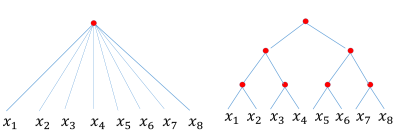
\includegraphics[scale=2.5]{../images/ComplexityNN.png}
\end{center}

\begin{itemize}
  \item $W_m^n$: class of $n$-variable functions with partial derivatives up to $m$-th order

  \item $W_m^{n,2}\subset W_m^n$: compositional subclass following binary tree structure

\end{itemize}

\textbf{Theorem.} Let $\sigma: \mathbb{R} \rightarrow \mathbb{R}$ be infinitely differentiable, and not a polynomial. For $f \in W_m^n$ the complexity of shallow networks that provide accuracy at least $\varepsilon$ is
$N=O\left(\varepsilon^{-n / m}\right)$ and is the best possible.\\ \\
\textbf{Theorem.} For $f \in W_m^{n, 2}$ consider a deep network with the same compositonal architecture and with an activation function $\sigma$ : $\mathbb{R} \rightarrow \mathbb{R}$ which is infinitely differentiable, and not a polynomial. The complexity of the network to provide approximation with accuracy at least $\varepsilon$ is

\begin{equation}
N=O\left((n-1) \varepsilon^{-2 / m}\right) .
\end{equation}

\textbf{Theorem.} Let $f$ be a L-Lipshitz continuous function of $n$ variables. Then, the complexity of a network which is a linear combination of ReLU providing an approximation with accuracy at least $\varepsilon$ is

$$
N_s=O\left(\left(\frac{\varepsilon}{L}\right)^{-n}\right)
$$

wheres that of a deep compositional architecture is

$$
N_d=O\left((n-1)\left(\frac{\varepsilon}{L}\right)^{-2}\right) .
$$

\section{Physics Informed Neural Networks (PINNs)}
Setting of the problem: consider $\Omega \subset \mathbb{R}^d$ and a PDE parametrized by $\lambda$ for the solution $u(x)$:
\[
    f\left(x; \dfrac{\partial u}{\partial x_1}, \dots, \dfrac{\partial u}{\partial x_d}; \dfrac{\partial^2 u}{\partial x_1 \partial x_1}, \dots, \dfrac{\partial^2 u}{\partial x_1 \partial x_d}, \dots, \dfrac{\partial^2 u}{\partial x_d \partial x_d}; \lambda\right) = 0, \hspace{0.5cm} x \in \Omega    
\]
And $\mathcal{B}(u,x) = 0$ on the boundary $\partial \Omega$. For time-dependent problems $t$ is considered as a special component of $x$ and $\Omega$ contains also the temporal domain. The IC are treated as a special type of Dirichlet BC on the spatio-temporal domain. 
The training set is:
\[
    \mathcal{T} = {x_1, x_2, \dots, x_{|\mathcal{T}|}} \text{ of size } |\mathcal{T}|    
\]
Residual points:
\[
    \mathcal{T}_f \subset \Omega \text{ and } |\mathcal{T}_b \subset \partial \Omega     
\]
Then, we have:
\[
    \mathcal{L}(\theta; \mathcal{T}) = w_f\mathcal{L}_f(\theta; \mathcal{T}_f) + w_b\mathcal{L}_b(\theta; \mathcal{T}_b)     
\]
Where
\[
    \mathcal{L}_f(\theta; \mathcal{T}_f) = \dfrac{1}{|\mathcal{T}_f|} \sum_{x \in \mathcal{T}_f} \left\|f\left(x; \dfrac{\partial u}{\partial x_1}, \dots, \dfrac{\partial u}{\partial x_d}; \dfrac{\partial^2 u}{\partial x_1 \partial x_1}, \dots, \dfrac{\partial^2 u}{\partial x_1 \partial x_d}, \dots, \dfrac{\partial^2 u}{\partial x_d \partial x_d}; \lambda\right)\right\|^2_2 
\]
\[
    \mathcal{L}_b(\theta; \mathcal{T}_b) = \dfrac{1}{|\mathcal{T}_b|} \sum_{x \in \mathcal{T}_b} \left\|\mathcal{B}(u,x)\right\|^2_2
\]
\begin{center}
    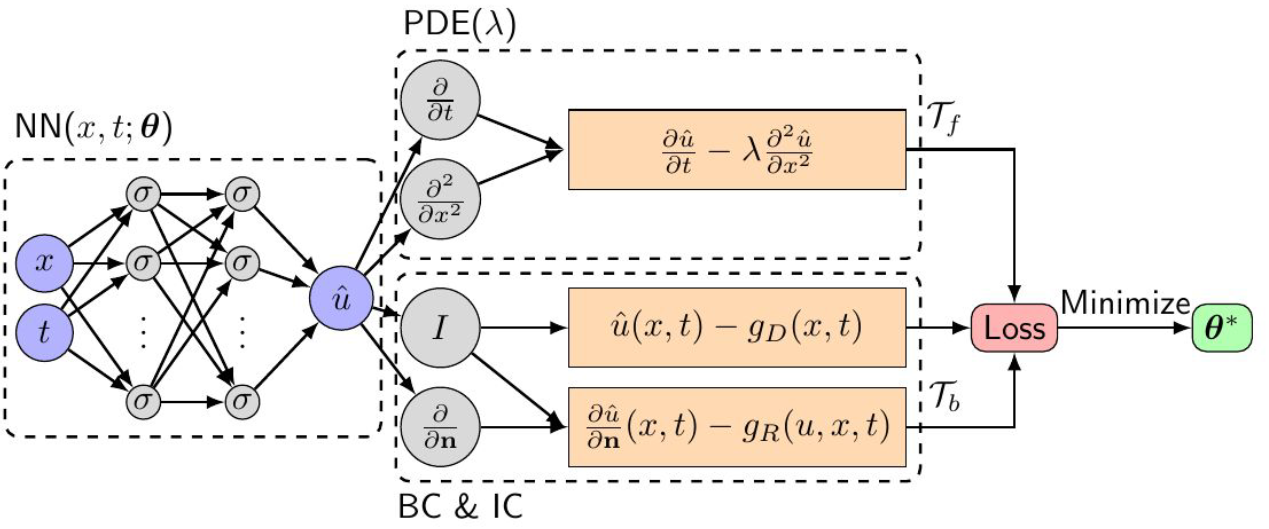
\includegraphics[scale=0.3]{../images/PINN_Architecture.png}
\end{center}
The actual PINN algorithm:
\begin{center}
    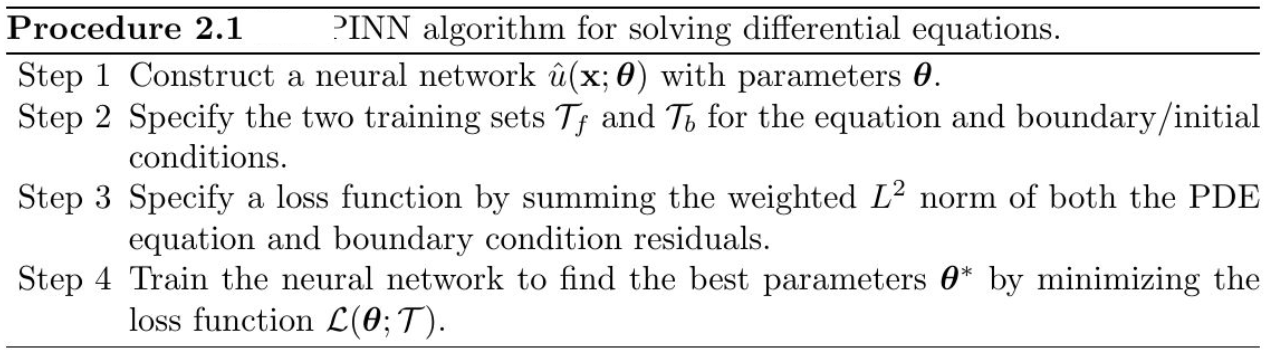
\includegraphics[scale=0.3]{../images/PINN_Algorithm.png}
\end{center}

\subsection*{Errors}
We define:
\begin{itemize}
    \item $\mathcal{F}$: family of all functions that can be represented by the chosen NN
    \item $u_{\mathcal{F}} = \arg \min_{f \in \mathcal{F}} \|f-u\|$: best function in $\mathcal{F}$ close to $u$
    \item $u_{\mathcal{T}} = \arg \min_{f \in \mathcal{F}} \mathcal{L}(\theta; \mathcal{T})$: solution given by the NN when the loss is at global minimum
    \item $\tilde{u}_{\mathcal{T}}$ = approximate solution returned by the optimizer
    \item $\varepsilon_{app}$: measures how closely $u_{\mathcal{F}}$ can approximate $u$
    \item $\varepsilon_{gen}$: is determined by the number and locations of residual points and by the capacity of the family $\mathcal{F}$
    \item $\varepsilon_{opt}$: is due to the loss function complexity and the optimization setup (learning rate, number of iterations, \dots)
\end{itemize}

\[
    \varepsilon := \|\tilde{u}_{\mathcal{T}} - u\| \leq \underbrace{\|\tilde{u}_{\mathcal{T}} - u_{\mathcal{T}}\|}_{\varepsilon_{opt}} + \underbrace{\|u_{\mathcal{T}} - u_{\mathcal{F}}\|}_{\varepsilon_{gen}} + \underbrace{\|u_{\mathcal{F}} - u\|}_{\varepsilon_{app}}    
\]
\begin{center}
    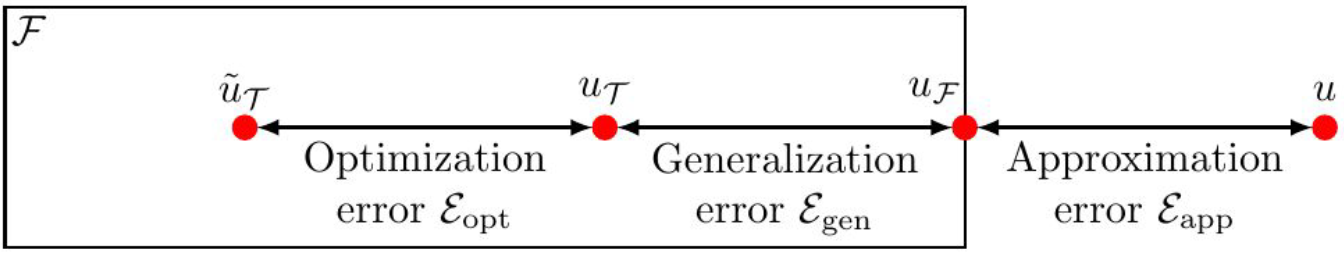
\includegraphics[scale=0.3]{../images/PINN_Error.png}
\end{center}
Comparison between PINN and FEM:
\begin{center}
    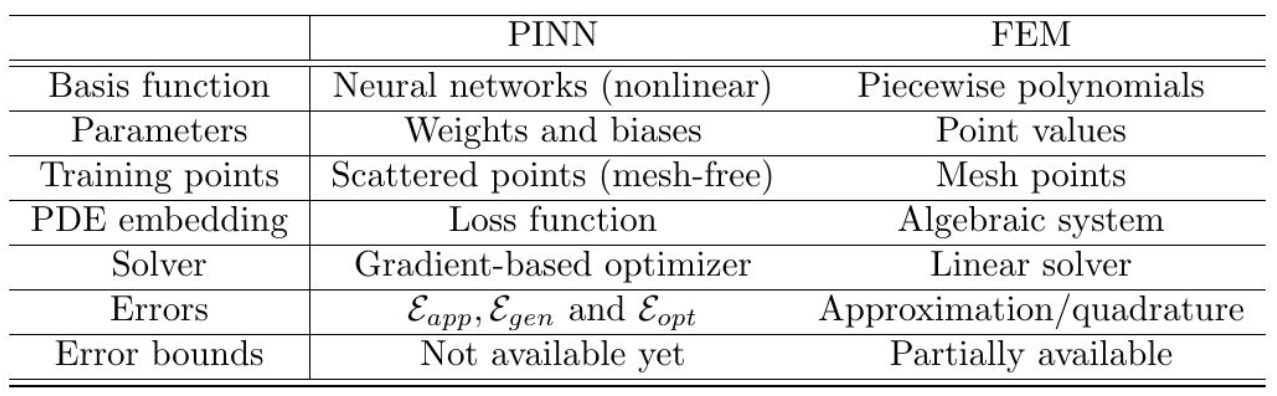
\includegraphics[scale=0.3]{../images/PINN_FEM_Comparison.png}
\end{center}

\subsection*{NS cylinder}
\[
    \begin{cases}
        \nabla \cdot u = 0 & x \in \Omega, t \in (0, T]\\
        \dfrac{\partial u}{\partial t} - \nu \nabla^2 u + (u \cdot \nabla)u + \nabla p = f & x \in \Omega, t \in (0, T]\\
    \end{cases}
\]
\begin{center}
    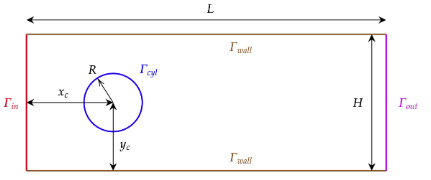
\includegraphics[scale=0.3]{../images/NS_Cylinder1.png}
\end{center}
\begin{center}
    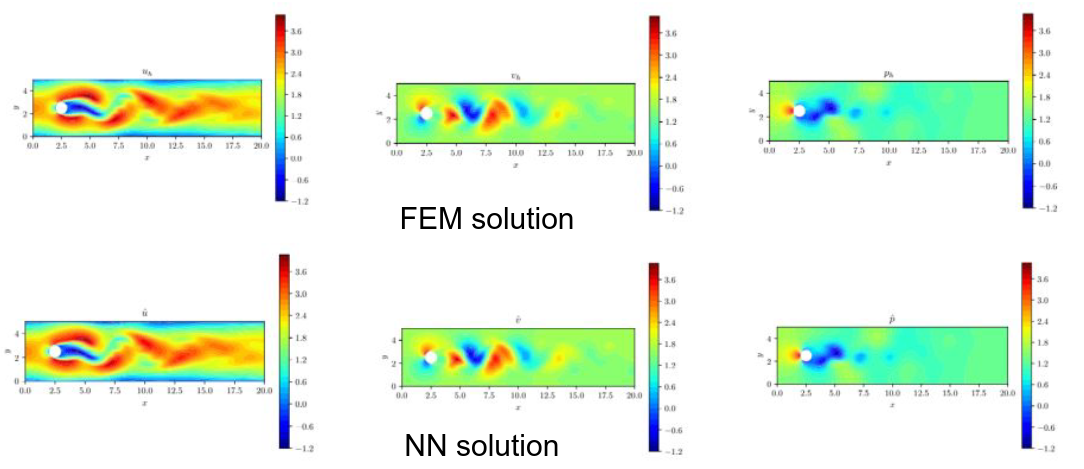
\includegraphics[scale=0.3]{../images/FEM_PINN_Solution.png}
\end{center}

\subsection*{PINNs for inverse problems}
Inverse problem: presence of unknown parameters $\lambda$ and some extra information on points $\mathcal{T}_i \subset \Omega$:
\[
    \mathcal{I}(u,x) = 0 \hspace{0.3cm}\text{for } x \in \mathcal{T}_i    
\]
\[
    \mathcal{L}(\theta, \lambda; \mathcal{T}) = w_f \mathcal{L}_f(\theta, \lambda; \mathcal{T}_f) + w_b \mathcal{L}_b(\theta, \lambda; \mathcal{T}_b) + w_i \mathcal{L}_i(\theta, \lambda; \mathcal{T}_i)    
\]
Where
\[
    \mathcal{L}(\theta, \lambda; \mathcal{T}_i) = \dfrac{1}{|\mathcal{T}_i|} \sum_{x \in \mathcal{T}_i} \left\|\mathcal{I}(\hat{u},x)\right\|^2_2
\]